\chapter{Champ magnétique $|h_i|$}
\label{sec_laser}

Certains systèmes qui favorisent une espèce de particules d'un côté de l'interface et une autre espèce de l'autre côté se retrouvent dans plusieurs expériences, par exemple une croissance de cristaux contrôlée par un champ optique\cite{} ou le forçage d'une phase dans une autre dans des expériences d'optofluidique\cite{delville}. Ces systèmes ont la particularité d'avoir une singularité dans le champ magnétique au niveau de l'interface, du genre 
\begin{align}
	B(y) = B \sgn(y)
\end{align}
 où l'interface est placée convenablement en $0$ et $B$ est l'intensité du champ magnétique. Dans le formalisme SOS, ce champ magnétique se traduit par 
\begin{align}
	B(h_i) = B |h_i|
\end{align}
Pour $B>0$, le potentiel a un minimum absolu en $0$, confinant ainsi l'interface. On s'attend à ce que plus le champ magnétique devienne élevé, plus l'interface devienne confinée. 

Nous discuterons brièvement à la fin du chapitre le cas où $B$ est négatif.


	\section{Modèle gaussien}

Un potentiel aussi complexe présente de nombreuses difficultés pour la diagonalisation. Une des difficultés provient du grand nombre de degrés de liberté du système. Afin de diminuer la complexité du calcul, supposons que l'interface soit continue, c'est-à-dire que l'interface au point $x$ soit notée $h(x)$. Cette interface n'est plus définie uniquement aux sites discrets $i$, puisque l'on s'intéresse aux propriétés mésoscopiques du système.

L'énergie du modèle SOS est directement dictée par $E = \sigma \mathcal{L}$, où $\sigma$ est la tension superficielle de notre interface et $\mathcal{L}$ la longueur totale de notre interface. Cette longueur correspond à la distance parcourue par un marcheur brownien le long de l'interface dans des conditions en $x$ périodiques. D'un point de vue continu, la distance effectuée pour de petits déplacements est $d\mathcal(L) = \sqrt{1+\frac{dh^2}{dx^2}} \simeq h'^2 $.
L'Hamiltonien discret correspondant devient gaussien
\begin{align}
    H = J \sum_i (h_i-h_{i+1})^2
\end{align}
tandis qu'une version continue du problème est 
\begin{align}
	H = \frac{\sigma}{2} \int_0^L h'^2(x) dx - B \int_0^L |h(x)|dx
\end{align}
Cet hamiltonien gaussien est très similaire à celui que l'on peut retrouver pour les ondes capillaires\cite{} et facilite grandement les calculs. 

    \section{Distribution de l'interface}

Pour une interface avec des conditions aux bords fixe $h(0) = h$ et $h(L) = h^\ast$, la fonction de partition est donnée par
\begin{align}
	\mZ(h,h^\ast,L) = \int_{h(0)=h} d[h] \delta(h(L)-h^\ast)e^{-\frac{\sigma}{2} \int_0^L h'^2(x) dx + B \int_0^L |h(x)|dx}
\end{align}
La configuration de l'interface à un instant $t$ est similaire à celle de la trajectoire temporelle d'un marcheur brownien commençant à $h(0)$ et finissant à $h(L)$\cite{}.
La fonction de partition $\mZ$ obéit alors à l'équation de Schrödinger temporelle
\begin{align}
	\frac{\partial \mZ}{\partial L} = \frac{1}{2 \beta \sigma} \frac{\partial^2 \mZ}{\partial h^2}  - B \beta |h| \mZ
\end{align}
avec la condition initiale $\mZ(h,h',0) = \delta(h-h')$.  En absence d'un potentiel externe on retrouve les solutions en sinus et cosinus décrivant une interface délocalisée à travers tout le système. En décomposant la fonction de partition dans la base des solutions stationnaires $\psi_E$ correspondant aux énergies propres $E$ 
\begin{align}
	Z(h,h',L) = \sum_E e^{-EL}\psi_E(h)\psi_E(h')
	\label{schro_temp}
\end{align}
À nouveau, dans la limite thermodynamique, seul l'état fondamental $E_0$ contribue à la distribution des hauteurs $p(h) = \psi_{E_0}^2(h)$.
Chaque fonction propre obéit alors à l'équation de Schrödinger 
\begin{align}
	\epsilon \psi_\epsilon = - \frac{1}{2} \frac{\partial^2 \psi_\epsilon}{\partial h^2} + \lambda |h| \psi_\epsilon
\end{align}
où l'équation a été admiensionalisée par $\epsilon = E\beta\sigma$ et $\lambda=\beta^2 \sigma B$.
Les solutions sont données par les fonctions d'ondes paires
\begin{align}
	\psi_\epsilon (h) = Ai \left( (2\lambda)^\frac{1}{3}|h|-\frac{\epsilon}{\lambda} \right)
\end{align}


où $Ai(x)$ est la fonction de Airy. Par analogie avec l'oscillateur harmonique quantique, nous cherchons des solutions avec des conditions aux limites $\psi'_\epsilon(0) = 0$ pour les états pairs et $\psi_\epsilon(0) = 0$ pour les états impairs. Cela nous donne $\epsilon_n = 2^{-\frac{1}{3}} \lambda^\frac{2}{3}\alpha_n$ où $-\alpha_{2n} \greater 0$ est le 2n-ième zéro de la dérivée de la fonction d'Airy Ai' et $-\alpha_{2n+1} \greater 0$ est le (2n+1)-ième zéro de la fonction d'Airy Ai. L'état fondamental est donné par le plus petit zéro de la fonction $\alpha_0 = 1.0187..$ et a une énergie de 
\begin{align}
	E_0 = 2^{-\frac{1}{3}} \alpha_0 \beta^\frac{1}{3}\sigma^{\frac{1}{3}}B^\frac{2}{3}
\end{align}
L'état fondamental s'écrit alors
\begin{align}
	\psi_0(h) = \frac{ Ai ( (2\lambda)^\frac{1}{3} |h|-\alpha_0 )}{ \sqrt{2 \int_0^\infty dh Ai^2 ( (2\lambda)^\frac{1}{3} |h|-\alpha_0 ) }}
\end{align}
où le terme d'en bas est une constante de normalisation utilisant la symétrie $p(h)=p(-h)$.  
On peut calculer les états excités suivants suivant leur parité, les états pairs s'écrivant
\begin{align}
	\psi_{2n}(h) = \frac{ Ai ( (2\lambda)^\frac{1}{3} |h|-\alpha_{2n} )}{ \sqrt{2 \int_0^\infty dh Ai^2 ( (2\lambda)^\frac{1}{3} h-\alpha_{2n} ) }}
\end{align}
et les états impairs
\begin{align}
	\psi_{2n+1}(h) = \frac{ \sgn(h) Ai ( (2\lambda)^\frac{1}{3} |h|-\alpha_{2n+1} )}{ \sqrt{2 \int_0^\infty dh Ai^2 ( (2\lambda)^\frac{1}{3} h-\alpha_{2n+1} ) }}
\end{align}
d'énergie $E_{n} = E_0 \frac{\alpha_{n}}{\alpha_0}$. 

\begin{figure}[h]
	\begin{minipage}[t]{0.5\linewidth}
        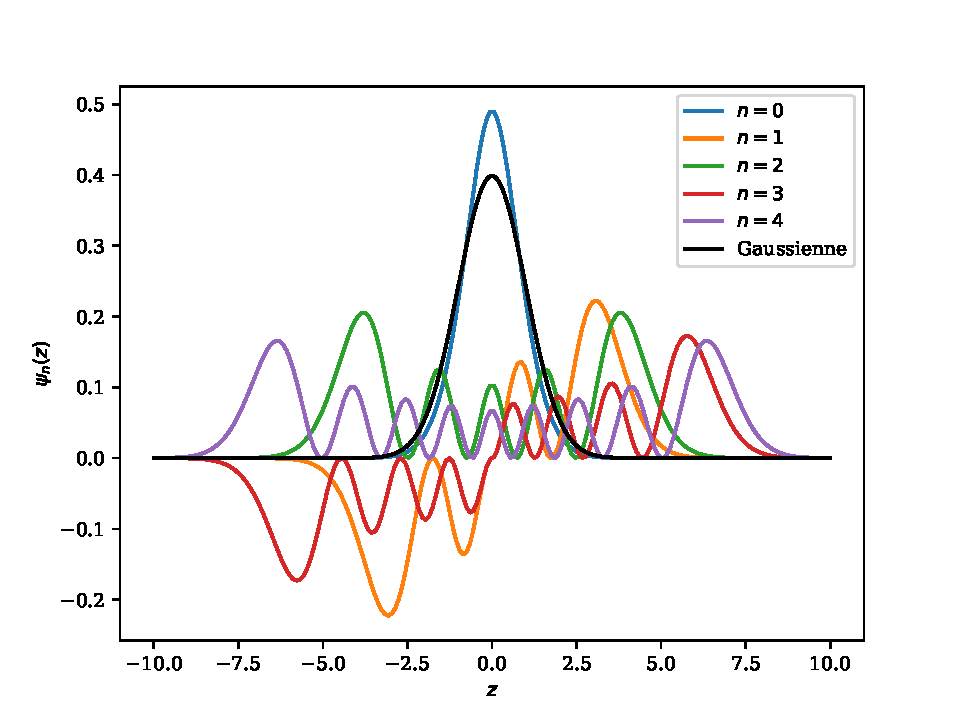
\includegraphics[width=\linewidth]{sosequi-laser/etats-laser.pdf}
	\end{minipage}%
	\begin{minipage}[t]{0.5\linewidth}
    	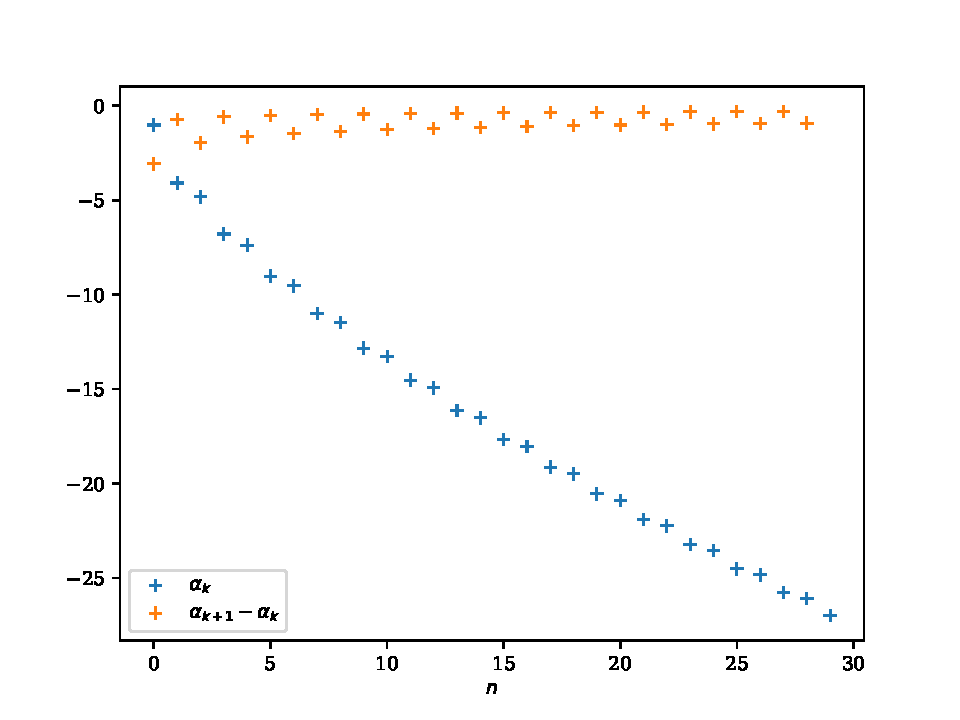
\includegraphics[width=\linewidth]{sosequi-laser/energies-laser.pdf}
	\end{minipage}
    \caption{À gauche, états propres $\psi_n$ avec en noir, une référence par rapport à la distribution gaussienne. À droite, la série $\alpha_n$.}
\end{figure}



On peut adimensionner la distribution des hauteurs par $z = (2\lambda)^\frac{1}{3}h$, et on peut définir une largeur caractéristique de l'interface 
\begin{align}
	\xi_\perp = \frac{1}{(2\beta^2 \sigma B)^\frac{1}{3}}
	\label{xi_perp}
\end{align}


La distribution des hauteurs dans un système infini devient 
\begin{align}
	p(z) = \psi_0^2(z) = \frac{ Ai^2 ( |z|-\alpha_0 )}{ 2 \int_0^\infty dz Ai^2 ( z-\alpha_0 ) }
	\label{airy}
\end{align}
	
\begin{figure}[h]
	\begin{minipage}[t]{0.5\linewidth}
		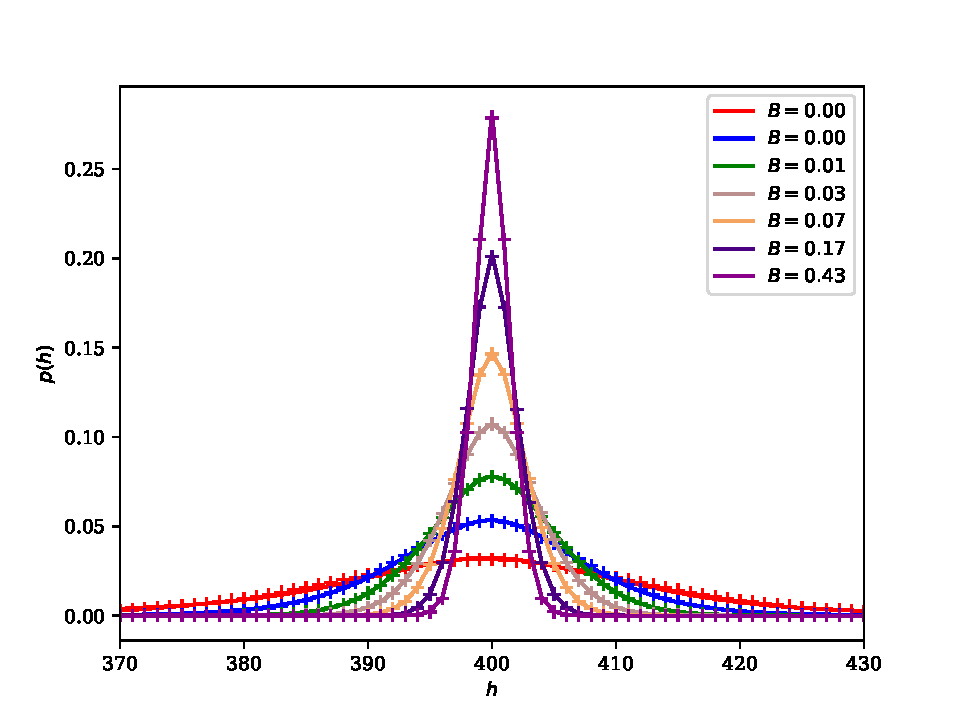
\includegraphics[width=\linewidth]{sosequi-laser/histo.pdf}
	\end{minipage}%
	\begin{minipage}[t]{0.5\linewidth}
		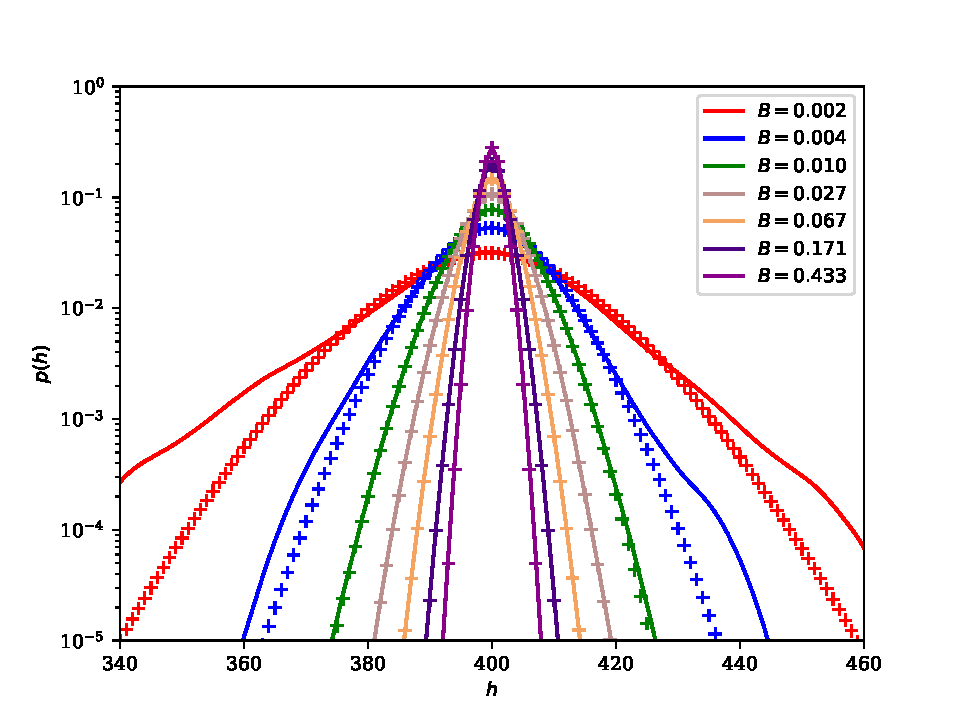
\includegraphics[width=\linewidth]{sosequi-laser/loghisto.pdf}
	\end{minipage}
	\caption{ Distribution de l'interface à $\beta = \beta_C$ autour d'un système centré à $L_Y=400$ en ligne et un fit selon la distribution de Airy \ref{airy}\protect\footnotemark en croix en échelle normale (à gauche) et en échelle log (à droite). Les écarts aux grandes fluctuations sont dues à un temps d’échantillonnage trop faible ($10^8$ MC steps) par rapport au temps de corrélation ($T_{cor} \simeq 100$), ce qui ne donne qu'environ $10^6$ états décorrélés. Par comparaison, à haut champ magnétique, le temps de corrélation est $T_{cor} \simeq 2$.  }
	\label{histo_airy}
\end{figure}

\footnotetext{En C++, les tableaux commençant par l'indice $0$, il est donc plus simple de centrer le système loin de $0$ afin de ne pas avoir à translater les variables à chaque fois. Par ailleurs, le fit est très sensible aux conditions initiales.}

\begin{figure}[h]
	\begin{minipage}[t]{0.5\linewidth}
		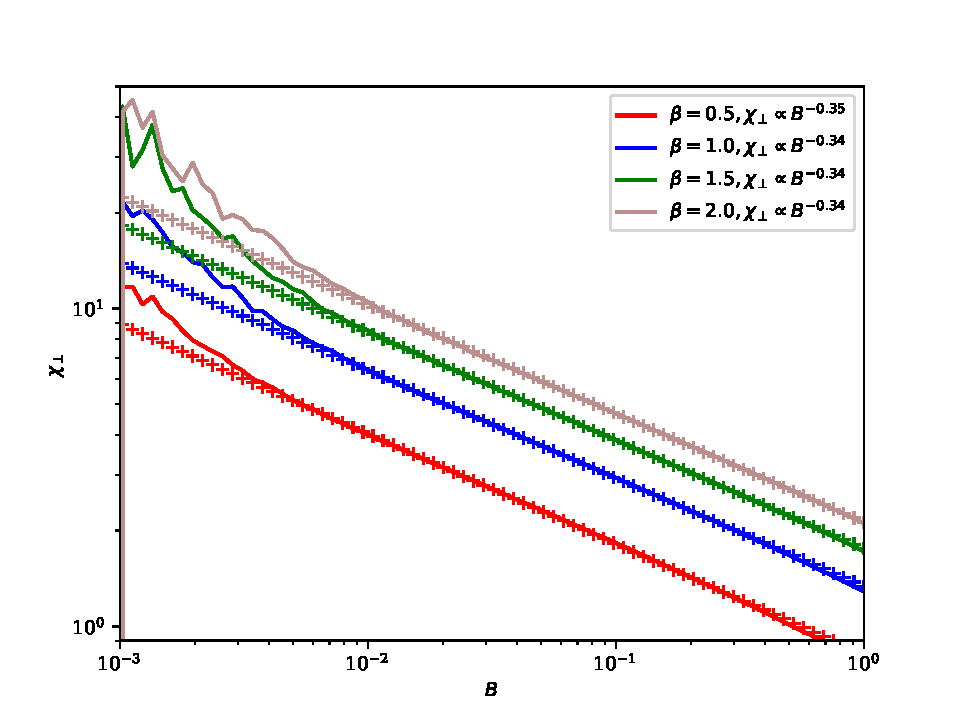
\includegraphics[width=\linewidth]{sosequi-laser/glau-chi.pdf}
	\end{minipage}%
	\begin{minipage}[t]{0.5\linewidth}
		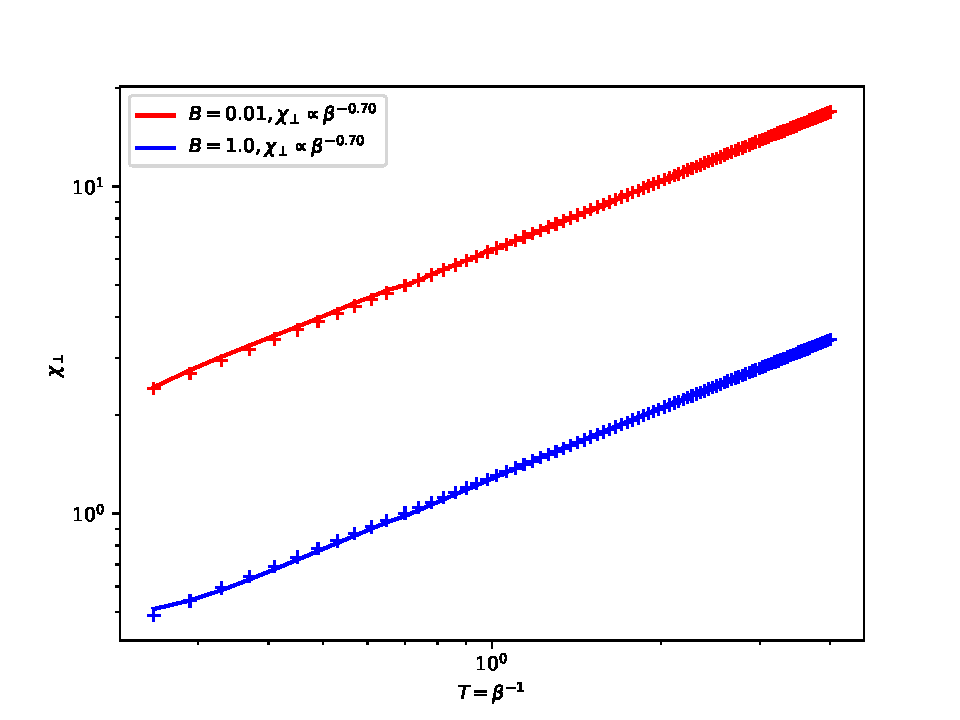
\includegraphics[width=\linewidth]{sosequi-laser/glau-chi-temp.pdf}
	\end{minipage}
	\caption{$\xi_\perp$ calculé via un fit de la distribution numérique par la distribution de Airy après $10^8$ MC steps (\ref{airy}) en fonction du champ magnétique et à température constante (gauche) ou en fonction de la température et à champ magnétique constant (droite). Les fluctuations pour $B$ petit s'expliquent par la difficulté d'équilibrage du système. On retrouve une loi en puissance comme dans l'équation \ref{xi_perp}.}
	\label{expo_airy}
\end{figure}

Comme montré précédemment, le calcul numérique de la distribution de l'interface nous permet d'avoir accès à  la tension de surface de notre modèle via la mesure de la longueur caractéristique $\xi_\perp$. Dans la figure \ref{histo_airy}, le fit de la distribution des hauteurs via l'équation \ref{airy} nous permet d'obtenir $\xi_\perp(\beta,B)$ de la figure \ref{expo_airy}. Ainsi, on obtient que 
\begin{align}
	\xi_\perp(\beta,B) \propto \beta^{-0.34} B^{-0.70} 
\end{align}

\textbf{Est-ce utile de faire une étude plus poussée sur plus de B et $\beta$ afin d'avoir une barre d'erreur sur les exposants ?}

Grâce aux calculs, il est possible d'inverser \ref{xi_perp} afin de trouver numériquement la tension superficielle du système. Dans le tableau \ref{tab_sigma}, en supposant un exposant en $\beta$ de $-0.70$, un tableau à titre informatif sur la tension de surface calculée en fonction de différents paramètres $T = \frac{1}{\beta}$ et $B$ grâce à l'équation \ref{xi_perp}. Les grandes fluctuations de $\sigma$ proviennent d'un échantillonage trop faible du calcul de l'exposant de $\beta$ et de $B$. De plus, d'après la figure \ref{expo_airy}, il semblerait que la loi en puissance ne soit pas valable dans tous les régimes, ce qui ajoute de l'incertitude à nos calculs.
Au final on constate que $\sigma \simeq 4.5$ dans notre modèle pour $J=1$. Des études plus approfondies utilisant la fonction de corrélation et $\xi_\parallel$ permettraient calculer précisément la tension superficielle dans le modèle SOS.

\begin{table}[h]
    \centering
$\begin{array}{|c|c|c|c|c|}
\hline
    T & B & \xi_\perp & \text{Exposant de B} &  \sigma \\
\hline
0.5 & 0.01 & 3.94 & -0.347 & 4.55 \\
0.5 & 1.0 & 0.78 & -0.347 & 4.01 \\
1.0 & 0.01 & 6.29 & -0.340 & 4.80 \\
1.0 & 1.0 & 1.28 & -0.340 & 4.23 \\
1.5 & 0.01 & 8.36 & -0.340 & 4.75 \\
1.5 & 1.0 & 1.72 & -0.340 & 4.36 \\
2.0 & 0.01 & 10.26 & -0.342 & 4.71 \\
2.0 & 1.0 & 2.11 & -0.342 & 4.37 \\
\hline
\end{array}$
    \caption{Meilleure estimation possible de la tension superficielle d'après les simulations numériques pour quelques valeurs de $T$ et de $B$.  }
    \label{tab_sigma}
\end{table}

    \section{Fonction de corrélation }

On peut également calculer la fonction de corrélation à deux-points. 
D'après l'éq \ref{schro_temp}, l'énergie de chaque état est une longueur caractéristique de chaque mode, $E_0$ étant la plus importante contribution au système. La longueur de corrélation parallèle à l'interface étant de l'ordre de grandeur de $E_0^{-1}$, on a 
\begin{align}
	\xi_\parallel = \frac{1}{E_0} =  2^\frac{1}{3}  \beta^{-\frac{1}{3}} \sigma^{-\frac{1}{3}}B^{-\frac{2}{3}}
\end{align}


Dans la limite thermodynamique $L$ grand, la fonction de corrélation  à l'interface est
\begin{align}
	C_f(r) &= \langle f(h(0))f(h(r))\rangle - <f(h(0))><f(h(r))>
\end{align}
Puisque nous sommes dans la limite thermodynamique, la fonction de partition devient $\mZ \simeq e^{-E_0 L}$ et $<f(h(0))> = <f(h(r))> = \int_{-\infty}^\infty dh f(h) \psi_0(h)^2 $.
On obtient alors que
\begin{align}
	C_f(r) =  \sum_{n\neq 0}\left[\int_{-\infty} ^\infty dh\  f(h)\psi_n(h)\psi_0(h)\right]^2\exp(-[\alpha_n-\alpha_0] \frac{r}{\xi_{||}})
\end{align}
En particulier, si
\begin{align}
	f(h) = {\rm sign}(h-y)
\end{align}
alors $C_f(r)=C(y,r)$ est la fonction de corrélation spin-spin mesurée parallèlement à l'interface à la hauteur $y$. On peut décomposer l'intégrale en deux parties, et grâce à un changement de variable obtenir
\begin{align}
	\int_{-\infty} ^\infty dh\  f(h)\psi_n(h)\psi_0(h)=  2\int_y ^\infty dh\  \psi_n(h)\psi_0(h)
\end{align}
Puisque les $\psi_n$ sont des fonctions d'onde orthogonales répondant à l'équation de Schrödinger, l'intégrale pour $n\neq 0$ est
\begin{align}
	I(n,y)&= \int_y^\infty dh\psi_n(h)\psi_0(h)  \nn
	&= \frac{1}{2}\frac{\psi_0(x)\psi'_n(y) - \psi_n(x)\psi_0'(y)}{\epsilon_n-\epsilon_0}
\end{align} 
Comme précédement, on notant $z= \frac{y}{\xi_\perp}$, on simplifie la fonction de corrélation en
\begin{align}
	C(z ,r) = \sum_{n\neq 0} \frac{\left[ Ai(|z|-\alpha_0)Ai'(|z|-\alpha_n) -Ai(|z|-\alpha_n)Ai'(|z|-\alpha_0) \right]^2}
{ \int_0^\infty dz Ai^2 ( z-\alpha_0 )2 \int_0^\infty dz Ai^2 ( z-\alpha_n ) (\alpha_n-\alpha_0)^2}e^{-[\alpha_n-\alpha_0] \frac{r}{\xi_{||}}}
\end{align}

La constante de normalisation peut être encore simplifiée. L'intégration par partie donne
\begin{align}
	N_n = \int_0^\infty dz Ai^2 (z -\alpha_n) = [z Ai^2 (z -\alpha_n)]_0^\infty - 2\int_0^\infty dz  z Ai(z -\alpha_n)Ai'(z -\alpha_n)
\end{align}
Le terme aux limites est nul, et en utilisant l'équation d'Airy 
\begin{align}
	Ai''(z) -z{\rm Ai}(z)=0 \implies z Ai(z-\alpha_n) = Ai''(z-\alpha_n) + \alpha_n Ai(z-\alpha_n)
\end{align}
on obtient
\begin{align}
	N_n &= -2\int_0^\infty dz [Ai''(z -\alpha_n)+\alpha_n Ai(z -\alpha_n)] Ai'(z -\alpha_n)  \nn
	&= Ai'^2(-\alpha_n) + \alpha_n Ai^2(-\alpha_n).
\end{align}

Cela nous donne au final
\begin{align}
	C(z,r) = \frac{1}{6.7 \times 10^{-3}}\sum_{n\neq 0} \frac{\left[ Ai(|z|-\alpha_0)Ai'(|z|-\alpha_n) -Ai(|z|-\alpha_n)Ai'(|z|-\alpha_0) \right]^2}
{(Ai'^2(-\alpha_n) + \alpha_n Ai^2(-\alpha_n))  (\alpha_n-\alpha_0)^2}e^{-[\alpha_n-\alpha_0] \frac{r}{\xi_{||}}}
\end{align}

À grande distance, seul le terme premier état excité $n=1$ contribue à la fonction de corrélation, ce qui nous donne
\begin{align}
C(x,r) \approx \frac{[{\rm Ai}\left(\frac{|x|}{\xi_{\perp}} -\alpha_{0}\right){\rm Ai}'\left( \frac{|x|}{\xi_{\perp}}-\alpha_{1}\right)-{\rm Ai}\left(\frac{|x|}{\xi_{\perp}} -\alpha_{1}\right){\rm Ai}'\left(\frac{|x|}{\xi_{\perp}} -\alpha_{0}\right)]^2}{\left[ {\rm Ai}'^2(-\alpha_{1}) \alpha_0 {\rm Ai}^2(-\alpha_0)\right](\alpha_1-\alpha_0)^2}\exp(-[\alpha_1-\alpha_0] \frac{r}{\xi_{||}}).
\end{align}

This is still quite complicated but if we restrict attention to $x=0$ we find
\begin{align}
C(0,r) \approx \frac{1}{(\alpha_1-\alpha_0)^2\alpha_0}\exp(-[\alpha_1-\alpha_0] \frac{r}{\xi_{||}}).
\end{align}
However at $x=0$ we can actually do better using the boundary conditions
that ${\rm Ai}(-\alpha_{2n+1}) =0$ and ${\rm Ai}'(-\alpha_{2n}) =0$ to give
\begin{align}
C(0,r) = \sum_{n=0}^\infty \frac{1}{(\alpha_{2n+1}-\alpha_0)^2\alpha_0}\exp(-[\alpha_{2n+1}-\alpha_0] \frac{r}{\xi_{||}}).%
\end{align}
We know that $C(0,0)=1$ and so (unless there is a mistake in the calculations) we have the remarkable identity
\begin{align}
\sum_{n=0}^\infty \frac{1}{(\alpha_{2n+1}-\alpha_0)^2\alpha_0} = 1.
\end{align}

The above calculation has some strange consequences, we see that for all $x$ the correlation function for large $r$ 
decays as 
\begin{align}
A(\frac{x}{\xi_\perp})\exp(-[\alpha_1-\alpha_0] \frac{r}{\xi_{||}}),
\end{align}
where $A(x)$ is the $x$ dependent amplitude, so the correlation length at large $r$ is independent of the position
$x$, now going into the bulk this predicts that $\xi_{||} = \xi_b$ where $\xi_b$ is the bulk correlation length (but in the presence of the magnetic field). 


\begin{figure}[h]
	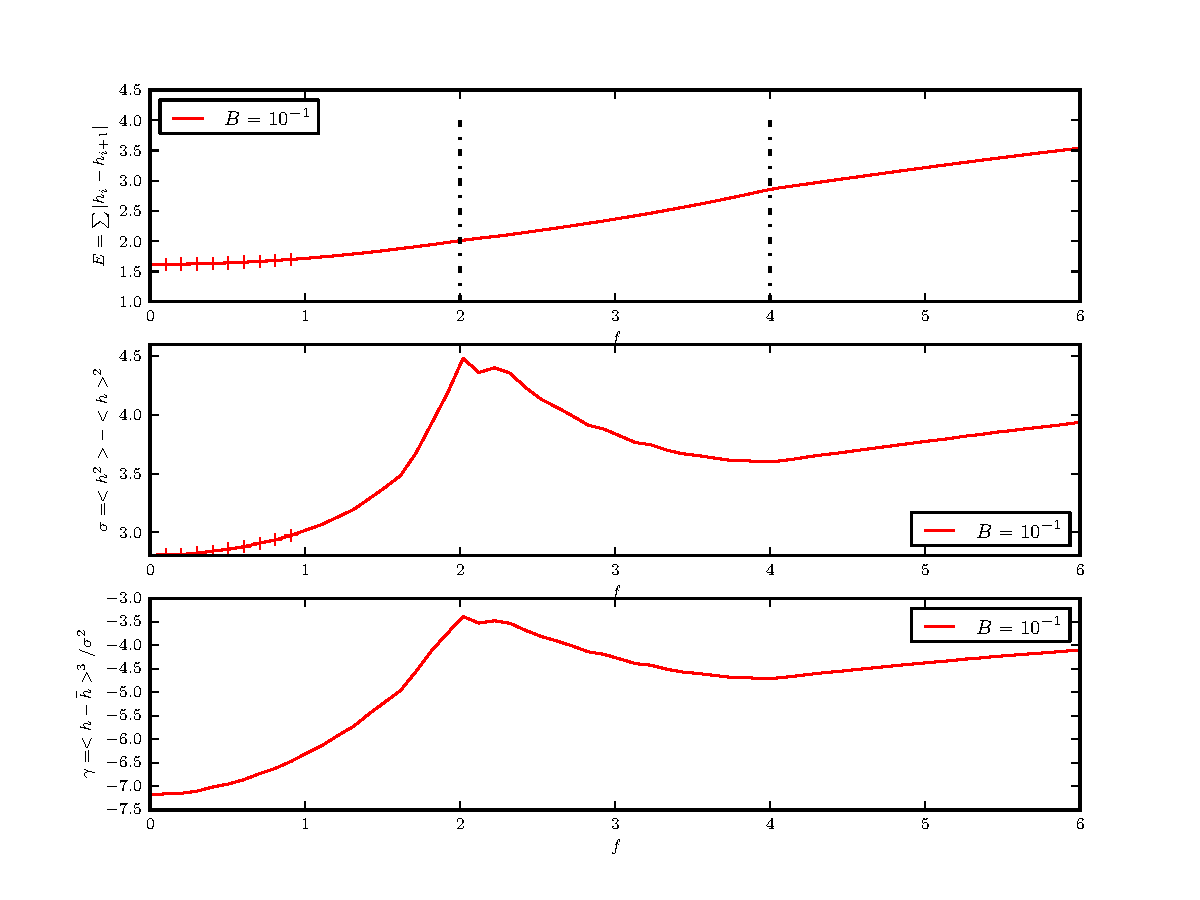
\includegraphics[width=\linewidth]{./sosequi-laser/sosj1.pdf}
	\caption{Énergie $E= \langle \sum_i |h_i-h_i+1| \rangle$ (en pointillé sa dérivée), variance $\sigma = \langle (H - \langle H \rangle )^2  \rangle$ et asymétrie $\gamma = \langle (H - \langle H \rangle )^3  \rangle / \sigma^2$ pour $B^0.1$. La magnétisation est constante et égale à $\langle H \rangle = 4.51$. Le temps de corrélation du système est presque constant en fonction du cisaillement $f$, allant de  $\tau(f=0) = 5.04$ à $\tau(f=6) = 5.00$ étapes de Monte Carlo. On note une brisure à $f=2J$ et $f=4J$.
Les croix notent un fit en carré pour petit $f$, montrant la symétrie du système par inversion du signe de $f$. }
\end{figure}

\begin{figure}
	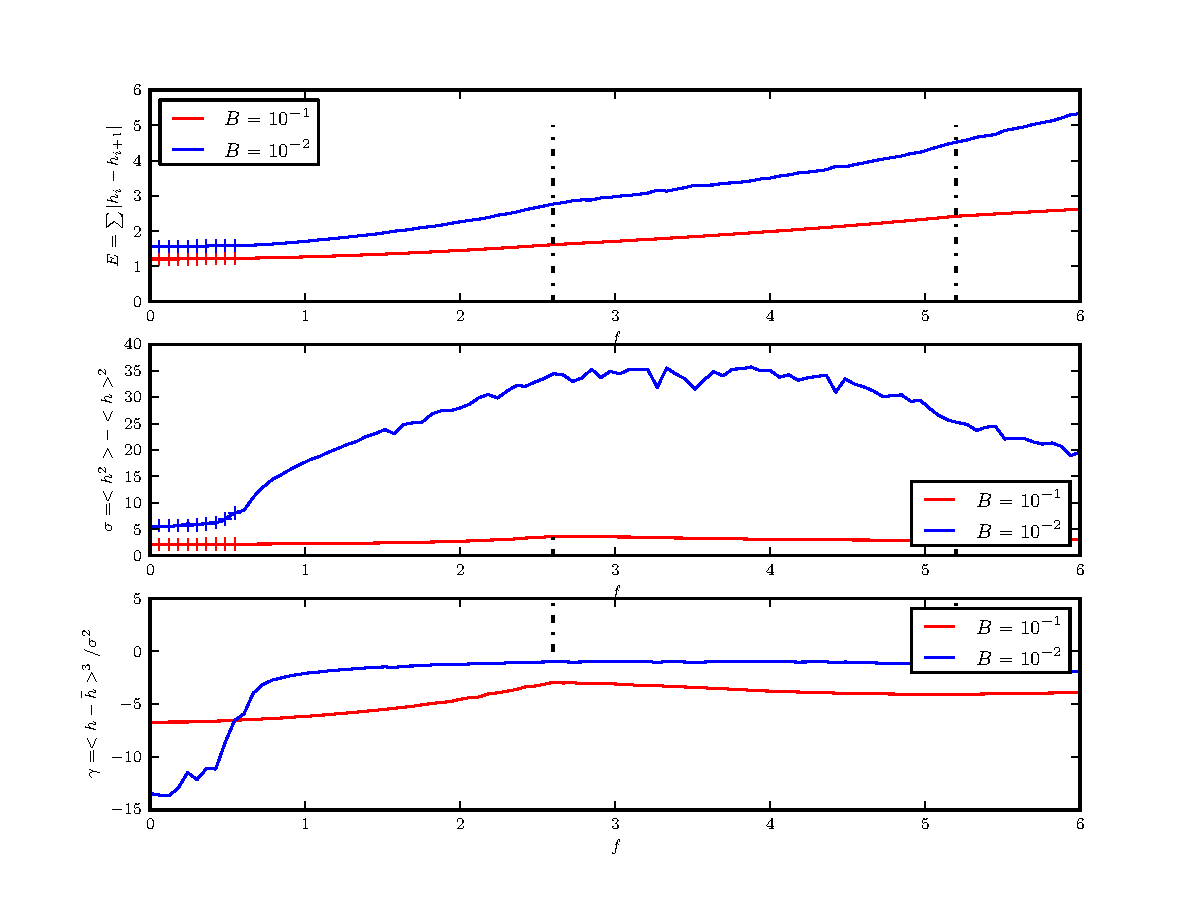
\includegraphics[width=\linewidth]{./sosequi-laser/j13.pdf}
	\caption{Same as before, with $J=1.3$ We observe a net inflexion in the energy at $2 J$ for  $B=0.01$ which corresponds to $<H>=11$. Nvertheless there is not threshold at $4 J = 5.2$. My guess is that the system is too far away from the boundary in order to interact strongly with it. Interstingly enough, for $B=0.1$, $<H>=3$ and we are too close to the boundaries to see anything.}
\end{figure}


\section{Cisaillement avec deux types de particules}

La construction naïve d'un modèle continu du cisaillement avec un seul type de particules ne donnera aucun résultat. En effet, pour que le cisaillement induise des effets hors équilibre, il faut que la dynamique des particules dans tout repère galilén soit le même. Si l'on considère une force de cisaillement uniforme qui induit la même vitesse moyenne sur toutes les particules du système, en nous plaçant dans un repère bougeant à la même vitesse que cette vitesse moyenne, nous retrouvons les mêmes propriétés à l'équilibre.
Afin de briser la symmétrie de translation, il faut soit induire un cisaillement non-uniforme, soit introduire des particules qui réagissent de manière différente vis-à-vis de cette force. Dans notre exemple sur les colloïdes, la gravité agit bien sur les polymères mais bien moins sur le solvant, ce qui brise en effet l'invariance galiléenne. 
Plusieurs études récentes portent sur le mouvement de systèmes avec plusieurs particules browniennes, incluant le problème des électrolytes étudié par Onsager \cite{onsager} il y a longtemps.

	\subsection{Discussion about the Gaussian model}
	
The Gaussian model has a stronger interaction, been as
\begin{align}
	\Delta E = J \sum (h'_i-h'_{i+1})^2 -(h_i-h_{i+1})^2+ f (i-j)
\end{align}
In this model the bond energy between two microstates can take any integer, as 
\begin{equation*}
	(h_i-h_j+2)^2 - (h_i-h_j)^2 = 4 (h_i-h_j+1)
\end{equation*}

The gaussian interaction is very strong, so we could expect a very smooth interface. The mean difference between two sites should be about $h_i-h_{i+1} \simeq 1$. In that case, the energy difference is discretized as ${-8,-4,0,4,8}$. 
Nonetheless we cannot predict exactly the same behaviour as in the SOS model because this approximation has to be verified everytime, which is false. 1

\begin{figure}
	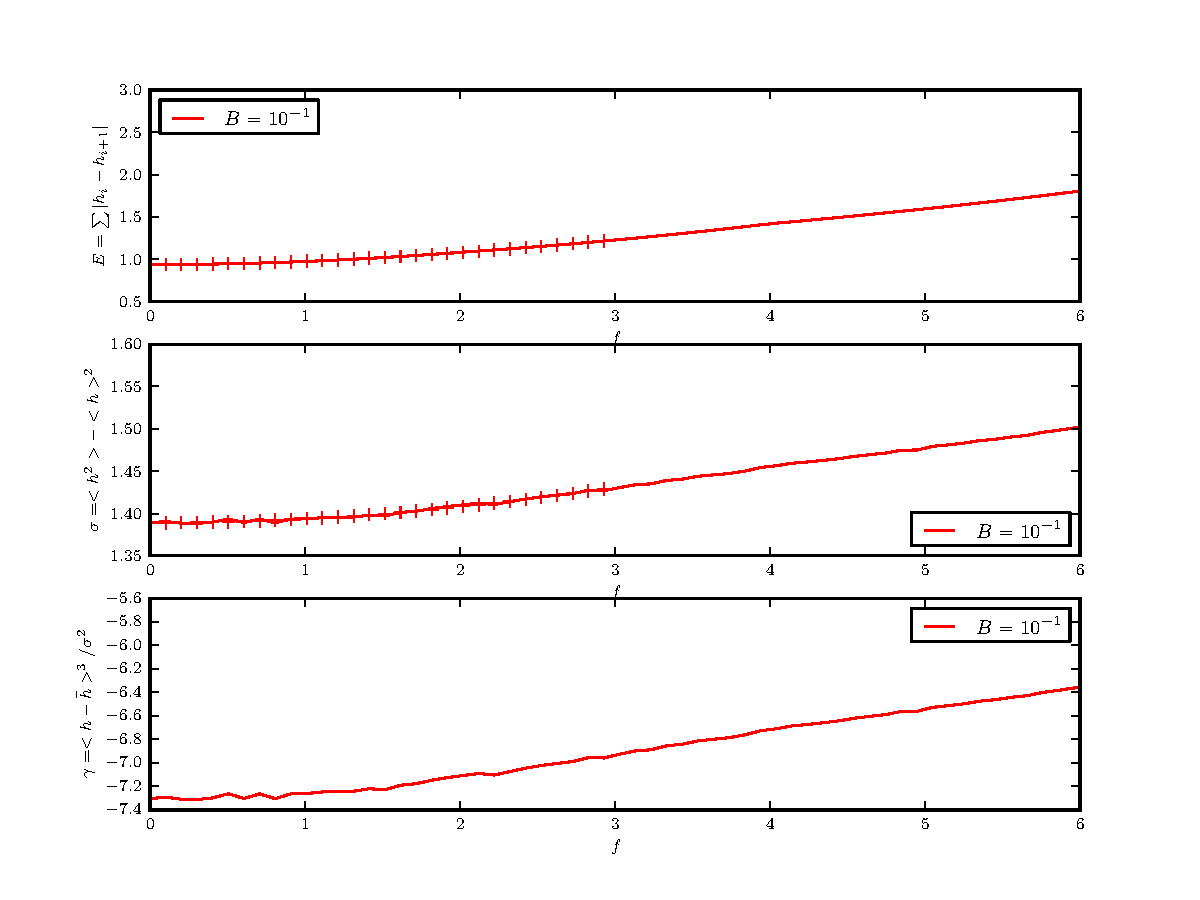
\includegraphics[width=\linewidth]{./sosequi-laser/gauss0.pdf}
	\caption{Bond energy, thickness (variance) and skewness of the interface for two different magnetic pressures. The magnetisation is constant and is equal to $<H>=2$ for $B=0.1$. As we are very close to the boundary, we see no threshold with the drive force. Simulations take longer with this model because the interaction is stronger}
\end{figure}


    \section{Conclusion}

Peu d'études permettent de relier les propriétés macroscopiques d'un système à sa dynamique moléculaire. Dans ce chapitre, nous avons réussi à calculer, via différentes méthodes, l'adéquation entre la théorie et un système discret que l'on a pu simuler. Un fit de nos données a permis de relever une valeur pour la tension superficielle pour le modèle SOS avec un hamiltonien gaussien et un champ magnétique agissant comme un laser. 